%%%%%%%%%%%%%%%%%%%%%%%%%%%%%%%%%%%%%%%%%
% Programming/Coding Assignment
% LaTeX Template
%
% This template has been downloaded from:
% http://www.latextemplates.com
%
% Original author:
% Ted Pavlic (http://www.tedpavlic.com)
%
% Note:
% The \lipsum[#] commands throughout this template generate dummy text
% to fill the template out. These commands should all be removed when 
% writing assignment content.
%
% This template uses a Perl script as an example snippet of code, most other
% languages are also usable. Configure them in the "CODE INCLUSION 
% CONFIGURATION" section.
%
%%%%%%%%%%%%%%%%%%%%%%%%%%%%%%%%%%%%%%%%%

%----------------------------------------------------------------------------------------
%	PACKAGES AND OTHER DOCUMENT CONFIGURATIONS
%----------------------------------------------------------------------------------------

\documentclass{article}
%\documentclass[11pt]{article}
\usepackage{fancyhdr} % Required for custom headers
\usepackage{lastpage} % Required to determine the last page for the footer
\usepackage{extramarks} % Required for headers and footers
\usepackage[usenames,dvipsnames]{color} % Required for custom colors
\usepackage{graphicx} % Required to insert images
\usepackage{subcaption}
\usepackage{listings} % Required for insertion of code
\usepackage{courier} % Required for the courier font
\usepackage{amsmath}
\usepackage{framed}

% Margins
\topmargin=-0.45in
\evensidemargin=0in
\oddsidemargin=0in
\textwidth=6.5in
\textheight=9.0in
\headsep=0.25in

\linespread{1.1} % Line spacing

% Set up the header and footer
\pagestyle{fancy}
\lhead{\hmwkAuthorName} % Top left header
\chead{\hmwkClass\ (\hmwkClassTime): \hmwkTitle} % Top center head
%\rhead{\firstxmark} % Top right header
\lfoot{\lastxmark} % Bottom left footer
\cfoot{} % Bottom center footer
\rfoot{Page\ \thepage\ of\ \protect\pageref{LastPage}} % Bottom right footer
\renewcommand\headrulewidth{0.4pt} % Size of the header rule
\renewcommand\footrulewidth{0.4pt} % Size of the footer rule

\setlength\parindent{0pt} % Removes all indentation from paragraphs

%----------------------------------------------------------------------------------------
%	CODE INCLUSION CONFIGURATION
%----------------------------------------------------------------------------------------

\definecolor{mygreen}{rgb}{0,0.6,0}
\definecolor{mygray}{rgb}{0.5,0.5,0.5}
\definecolor{mymauve}{rgb}{0.58,0,0.82}

\lstset{ %
  backgroundcolor=\color{white},   % choose the background color
  basicstyle=\footnotesize,        % size of fonts used for the code
  breaklines=true,                 % automatic line breaking only at whitespace
  captionpos=b,                    % sets the caption-position to bottom
  commentstyle=\color{mygreen},    % comment style
  escapeinside={\%*}{*)},          % if you want to add LaTeX within your code
  keywordstyle=\color{blue},       % keyword style
  stringstyle=\color{mymauve},     % string literal style
}

%----------------------------------------------------------------------------------------
%	DOCUMENT STRUCTURE COMMANDS
%	Skip this unless you know what you're doing
%----------------------------------------------------------------------------------------

% Header and footer for when a page split occurs within a problem environment
\newcommand{\enterProblemHeader}[1]{
%\nobreak\extramarks{#1}{#1 continued on next page\ldots}\nobreak
%\nobreak\extramarks{#1 (continued)}{#1 continued on next page\ldots}\nobreak
}

% Header and footer for when a page split occurs between problem environments
\newcommand{\exitProblemHeader}[1]{
%\nobreak\extramarks{#1 (continued)}{#1 continued on next page\ldots}\nobreak
%\nobreak\extramarks{#1}{}\nobreak
}

\setcounter{secnumdepth}{0} % Removes default section numbers
\newcounter{homeworkProblemCounter} % Creates a counter to keep track of the number of problems
\setcounter{homeworkProblemCounter}{0}

\newcommand{\homeworkProblemName}{}
\newenvironment{homeworkProblem}[1][Problem \arabic{homeworkProblemCounter}]{ % Makes a new environment called homeworkProblem which takes 1 argument (custom name) but the default is "Problem #"
\stepcounter{homeworkProblemCounter} % Increase counter for number of problems
\renewcommand{\homeworkProblemName}{#1} % Assign \homeworkProblemName the name of the problem
\section{\homeworkProblemName} % Make a section in the document with the custom problem count
\enterProblemHeader{\homeworkProblemName} % Header and footer within the environment
}{
\exitProblemHeader{\homeworkProblemName} % Header and footer after the environment
}

\newcommand{\problemAnswer}[1]{ % Defines the problem answer command with the content as the only argument
\noindent\framebox[\columnwidth][c]{\begin{minipage}{0.98\columnwidth}#1\end{minipage}} % Makes the box around the problem answer and puts the content inside
}

\newcommand{\homeworkSectionName}{}
\newenvironment{homeworkSection}[1]{ % New environment for sections within homework problems, takes 1 argument - the name of the section
\renewcommand{\homeworkSectionName}{#1} % Assign \homeworkSectionName to the name of the section from the environment argument
\subsection{\homeworkSectionName} % Make a subsection with the custom name of the subsection
\enterProblemHeader{\homeworkProblemName\ [\homeworkSectionName]} % Header and footer within the environment
}{
\enterProblemHeader{\homeworkProblemName} % Header and footer after the environment
}

%----------------------------------------------------------------------------------------
%	NAME AND CLASS SECTION
%----------------------------------------------------------------------------------------

\newcommand{\hmwkTitle}{Final Project} % Assignment title
\newcommand{\hmwkDueDate}{Sunday, Nov 25, 2018} % Due date
\newcommand{\hmwkClass}{CSC458} % Course/class
\newcommand{\hmwkClassTime}{LEC 5101} % Class/lecture time
\newcommand{\hmwkAuthorName}{Zhongtian Ouyang} % Your name
\newcommand{\hmwkAuthorID}{1002341012} % Your name

%----------------------------------------------------------------------------------------
%	TITLE PAGE
%----------------------------------------------------------------------------------------

\title{
\vspace{2in}
\textmd{\textbf{\hmwkClass:\ \hmwkTitle}}\\
\normalsize\vspace{0.1in}\small{Due\ on\ \hmwkDueDate}\\
\vspace{0.1in}
\vspace{3in}
}

\author{\textbf{\hmwkAuthorName}\\ \textbf{\hmwkAuthorID}}

\date{} % Insert date here if you want it to appear below your name

%----------------------------------------------------------------------------------------\
\begin{document}

\maketitle
\clearpage

%----------------------------------------------------------------------------------------
%	Common Tools
%----------------------------------------------------------------------------------------
%\begin{framed}
%\begin{lstlisting}[language=matlab]
%\end{lstlisting}
%\end{framed}

%\begin{figure}[h!]
%\centering
%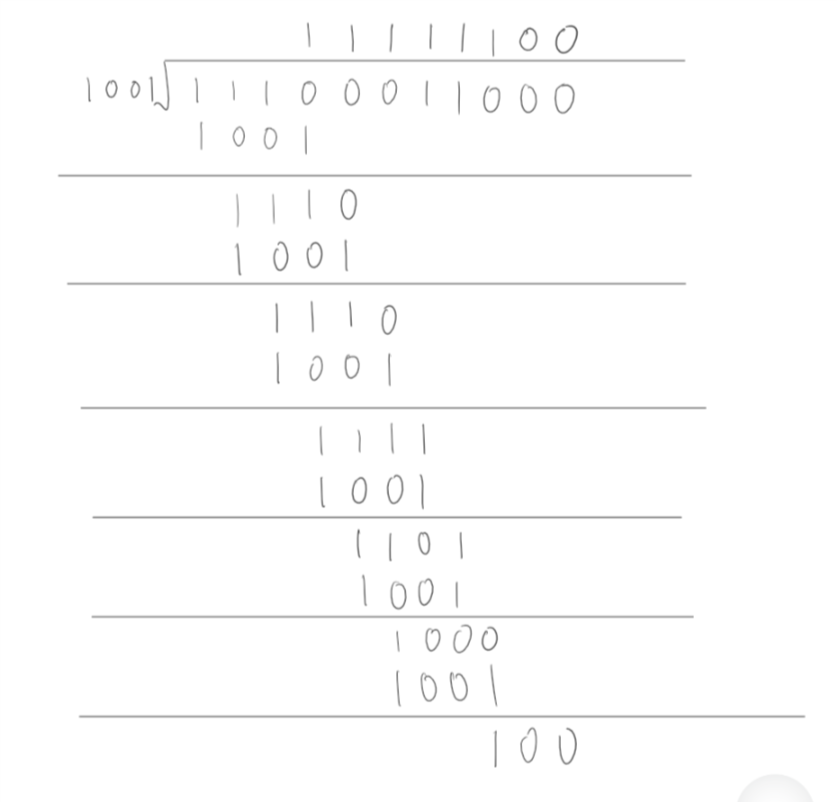
\includegraphics[width=0.6\linewidth]{q10a.png}
%\label{fig:q10a}
%\end{figure}\\

%\begin{figure*}[!ht]
%\begin{subfigure}{.5\textwidth}
% \centering
%  \includegraphics[width=.5\linewidth]{p4_1.JPG}
%  \caption{Full set}
%  \label{fig:sfig1}
%\end{subfigure}
%\begin{subfigure}{.5\textwidth}
% \centering
%  \includegraphics[width=.5\linewidth]{P4_2.JPG}
%  \caption{Two each}
%  \label{fig:sfig2}
%\end{subfigure}
%\caption{Part4 (a)}
%\label{fig:p4a}
%\end{figure*}
%----------------------------------------------------------------------------------------
%	Introduction
%----------------------------------------------------------------------------------------
Data used:
Student number end with 1012. (1012 + 0) \% 20 + 1 = 13\\
univ1\_pt13 is used\\

Resources used to complete the final project:\\
WireShark\\
Python: matplotlib, dpkt library\\

Citation:\\
For codes in modified\_pcap, they are copied from https://dpkt.readthedocs.io/en/latest/\_modules/dpkt/pcap.html. I modified the Reader class to store the pcap packet headers while reading packets from pcap\\

Reason for using logarithmic scale:\\
Many of the CDF charts use logarithmic scale for the x-axis because with logarithmic scale, we can see more details in the rapid increasing regions. This works especially well for the size charts. The reason is that packets and flows in the internet tend to clustered at the two end of chart so those cdf curves are very steep on the sides, while being flat in the middle. We are more interested in the steep part. Packets and flows that are only interchanging minimal informations tend to be very small, for example, ACK packets. While on the other hand, a file transfer could easily take multiple packets with a large size bounded by the MTU. I use log with base 2 in my graphs.
\clearpage
%----------------------------------------------------------------------------------------
%	PROBLEM 1
%----------------------------------------------------------------------------------------

% To have just one problem per page, simply put a \clearpage after each problem
\begin{homeworkProblem}

\noindent \textit{per-packet statistics}\\
The per-packet statistics are obtained using the per\_packet.py file. Notice that the statistic for IP doesn't contain ICMP and statistic for Ethernet contains ARP. Also, ICMP stats is a combine of ICMPv4 and ICMPv6.\\

The type of packets:\\
The total bytes field is the sum of packet's size for packets using each protocol.
\begin{table}[h!]
\begin{tabular}{llll}
                      & Count  & Percentage & Total Bytes \\
Ethernet              & 989027 & 100.00\%   & 487717605   \\
ARP                   & 80053  & 8.09\%     & 5129220     \\
IPV4                  & 859935 & 86.95\%    & 477298106   \\
IPV6                  & 15     & 0.00152\%    & 1650        \\
ICMP                  & 26328  & 2.66\%     & 1692408     \\
Other Network Layer   & 22696  & 2.29\%     & 3596221     \\
TCP                   & 608139 & 70.72\%    & 378995736   \\
UDP                   & 219174 & 25.48\%    & 78529873    \\
Other Transport Layer & 32637  & 3.80\%     & 19774147   
\end{tabular}
\end{table}

The size of packets:\\
The CDF charts are in the next page. Some analysis on the charts:\\
1. From the IP packets size's chart and Non-IP packets size's chart, we can see that packets using Non-IP protocols are usually very small, which means they are mostly used to interchange minimal informations, like ARP requests, not for large file transfers. On the other hand, IP packets' sizes are more spread-out. Notice that sizes are clustered around $2^6 = 64$ bytes and $2^10.5 \approx 1500$ bytes. This is a result from the two different kind of information packet want to transfer. Small ones for minimal, state informations. Large ones for file transfer.\\
2. Compare UDP's charts and TCP's charts, we can see some difference between the two protocols. The headers' sizes of UDP is much smaller than TCP headers' sizes, 8 compare to 20+. UDP has a lower overhead, while TCP headers contain more information and can support more complex algorithms for better reliability, etc. Also, UDP headers size are design to be fixed 8 bytes, while TCP headers' sizes can vary based on the options. The distribution of packet sizes is also different for UDP and TCP. For UDP, there are a lot more in the first half then in the second half, and a lot of packets have a size in the middle range. For TCP, the packet sizes are clustered at the two ends. Small packets are used for ACK, FIN, RST messages. Large packets for file transfer.\\
3. We can see that even though the IP header size can vary, almost all of them is 20. Also, the shape of all packets size is very similar to IP packets size bucause a major portion of all packets is using IP protocol as we can see from above table. This header graph only contains headers for IPv4. There are only very few IPv6 headers in the file.
\begin{figure*}[h]
\begin{subfigure}{.5\textwidth}
 \centering
  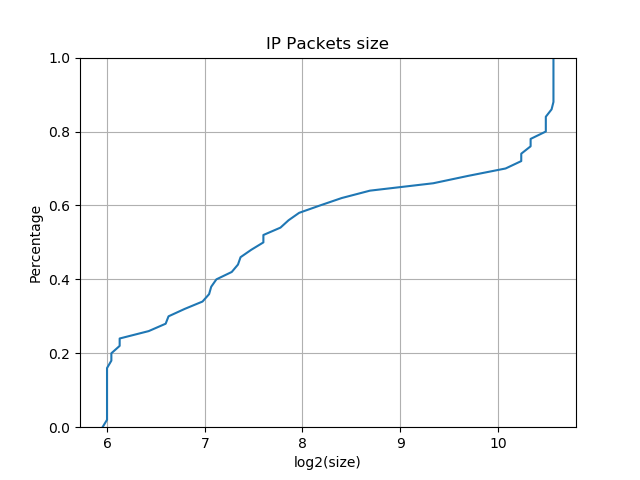
\includegraphics[width=0.9\linewidth]{graphs/IP_Packets_size.png}
\end{subfigure}
\begin{subfigure}{.5\textwidth}
 \centering
  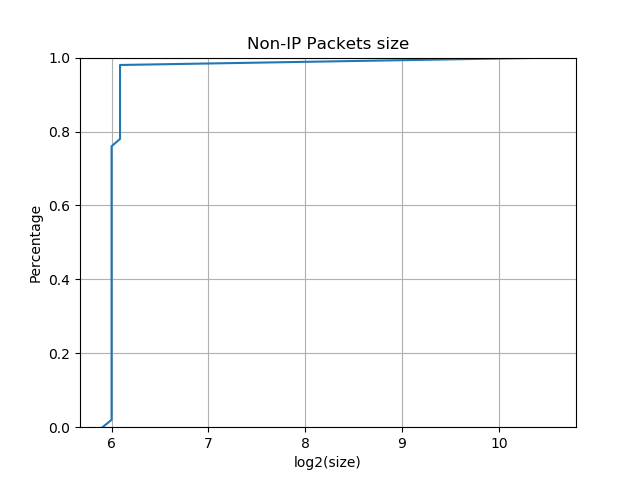
\includegraphics[width=0.9\linewidth]{graphs/Non-IP_Packets_size.png}
\end{subfigure}
\begin{subfigure}{.5\textwidth}
 \centering
  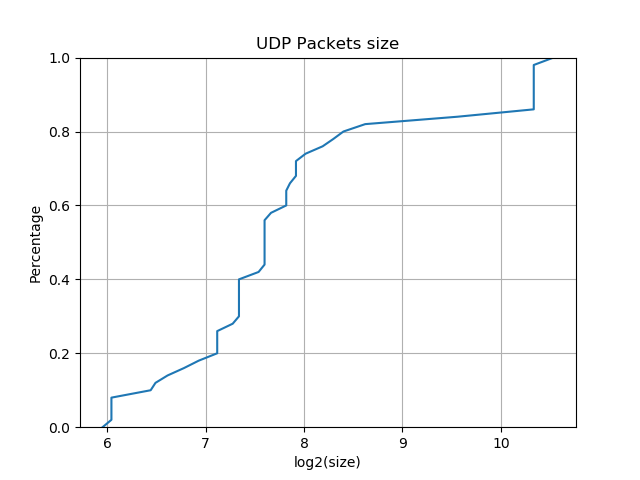
\includegraphics[width=0.9\linewidth]{graphs/UDP_Packets_size.png}
\end{subfigure}
\begin{subfigure}{.5\textwidth}
 \centering
  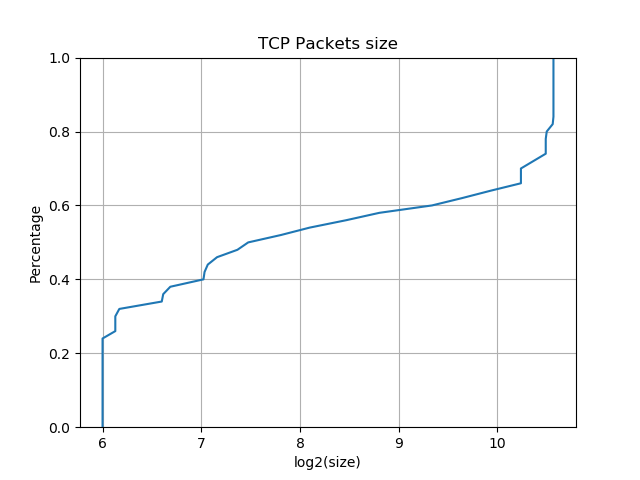
\includegraphics[width=0.9\linewidth]{graphs/TCP_Packets_size.png}
\end{subfigure}
\begin{subfigure}{.5\textwidth}
 \centering
  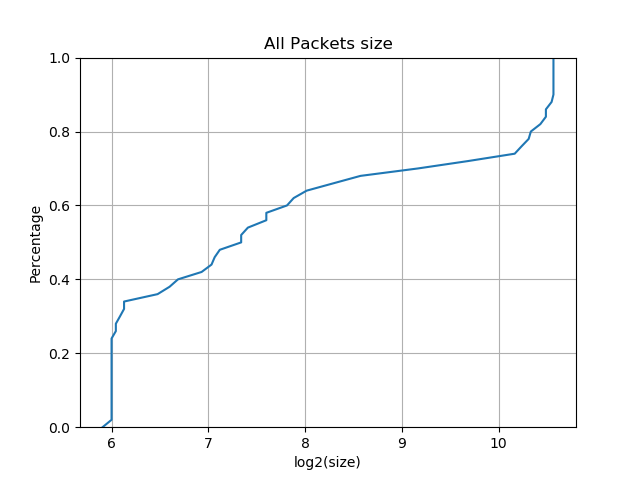
\includegraphics[width=0.9\linewidth]{graphs/All_Packets_size.png}
\end{subfigure}
\begin{subfigure}{.5\textwidth}
 \centering
  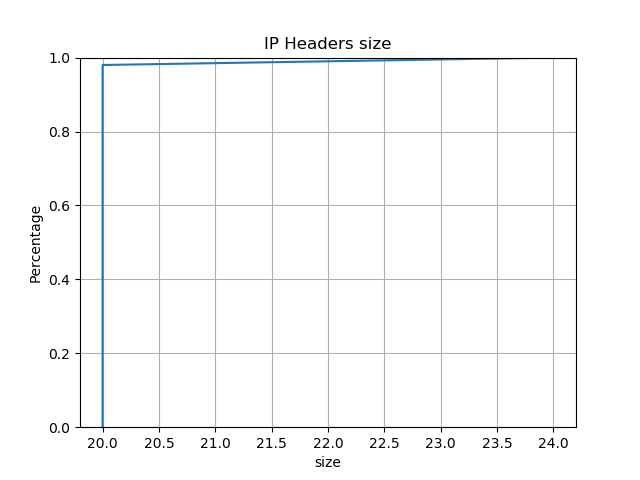
\includegraphics[width=0.9\linewidth]{graphs/IP_Headers_size.png}
\end{subfigure}
\begin{subfigure}{.5\textwidth}
 \centering
  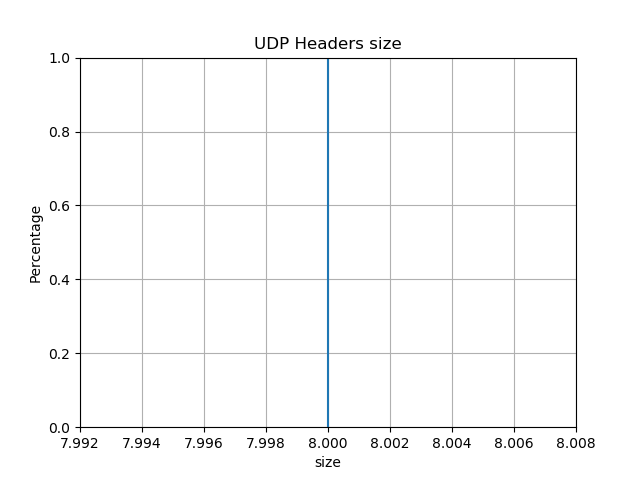
\includegraphics[width=0.9\linewidth]{graphs/UDP_Headers_size.png}
\end{subfigure}
\begin{subfigure}{.5\textwidth}
 \centering
  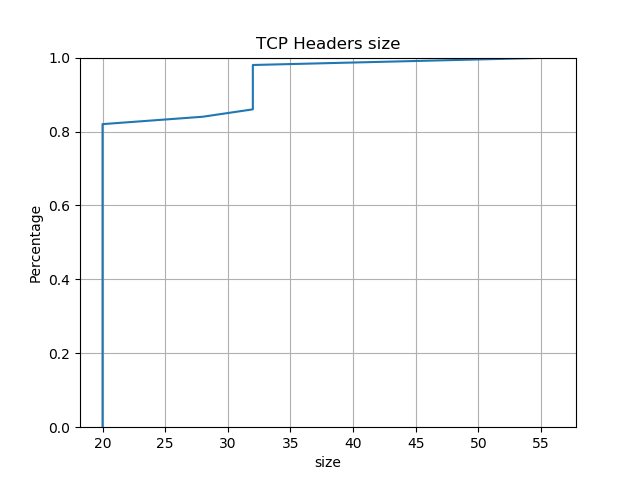
\includegraphics[width=0.9\linewidth]{graphs/TCP_Headers_size.png}
\end{subfigure}
\caption{Per Packet Statistics}
\label{per-packet}
\end{figure*}
\\
\end{homeworkProblem}
\clearpage
%----------------------------------------------------------------------------------------
%	PROBLEM 2
%----------------------------------------------------------------------------------------

\begin{homeworkProblem}
\noindent \textit{UDP and TCP flow statistics}\\

Flow Type:
\begin{table}[h!]
\begin{tabular}{llll}
                      & Count  & Percentage & Total Bytes \\
UDP flow           & 12252 & 56.40\%   & 78529873   \\
TCP flow               & 9473  & 43.60\%     & 378995736     
\end{tabular}
\end{table}

Flow Duration:\\
For both UDP and TCP flows, the flow durations have a similar distribution. Most of the flows have a very short duration, close to 0. And the max durations for both type of flows are 200+ seconds, which is the length of our pcap record. The only difference is that more TCP flows have a longer duration, about 20\%, while only less than 5\% UDP flows have a longer duration
\begin{figure*}[ht]
\begin{subfigure}{.33\textwidth}
 \centering
  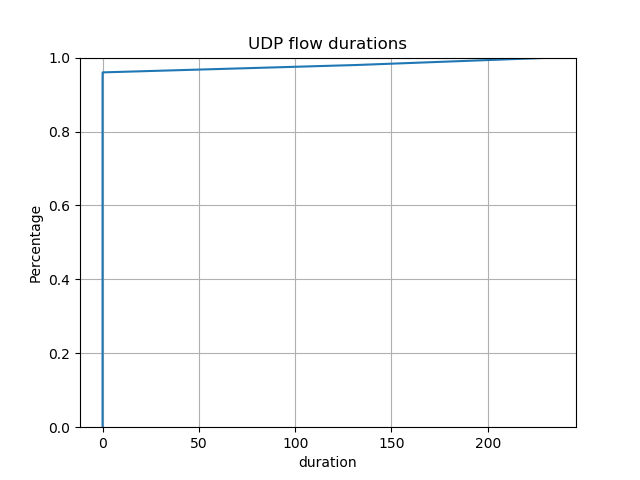
\includegraphics[width=1.1\linewidth]{graphs/UDP_flow_durations.png}
\end{subfigure}
\begin{subfigure}{.33\textwidth}
 \centering
  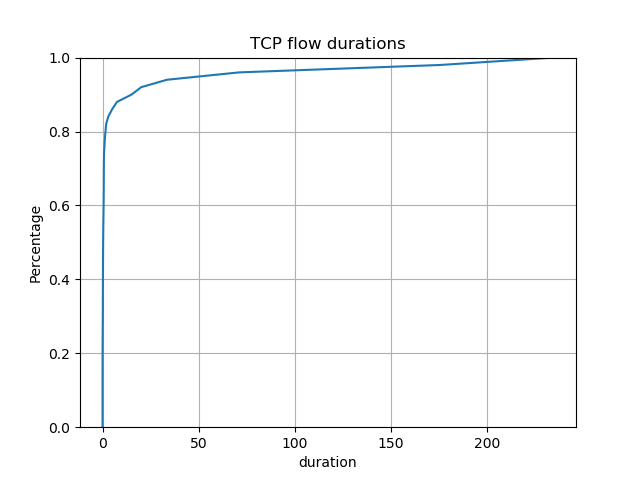
\includegraphics[width=1.1\linewidth]{graphs/TCP_flow_durations.png}
\end{subfigure}
\begin{subfigure}{.33\textwidth}
 \centering
  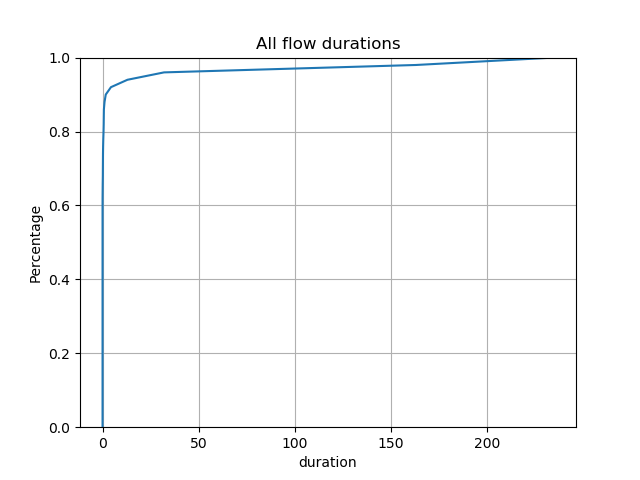
\includegraphics[width=1.1\linewidth]{graphs/All_flow_durations.png}
\end{subfigure}
\label{flow_duration}
\end{figure*}

Flow size:\\
The CDF charts for flow sizes are below. Compare the graphs using packet counts and the graph using bytes counts, we can see that each pair of graphs have a similar shape/distribution between them. If we compare the UDP graphs with TCP graphs, we can see that UDP flows' sizes are more clustered. A very big portion of UDP flows have only two packets and a small byte count. For TCP flows, their sizes are more spread out in the first half of the graph. Also, most flows have more than 5 packets because it need 3 packets for the handshake process, which also make TCP flows have larger byte counts. For the TCP overhead ratio, I calculate it as (all headers size)/(total tcp payload size). We can see that TCP is not very efficient. While generally the overhead ratio is between 1/16 and 1, about 20\% of tcp flows  didn't transfer any data.
\begin{figure*}[ht]
\begin{subfigure}{.5\textwidth}
 \centering
  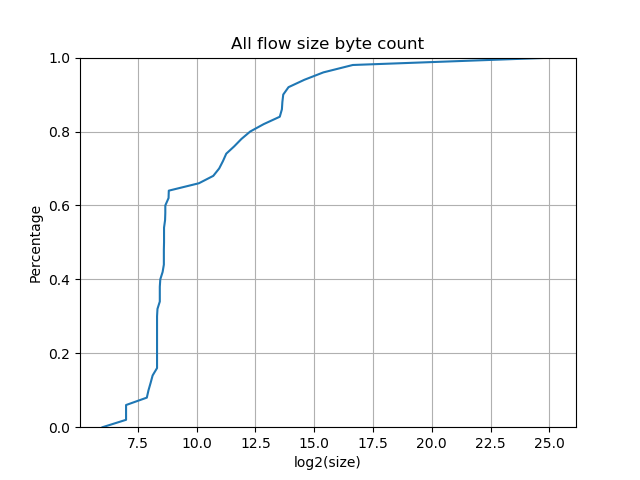
\includegraphics[width=0.9\linewidth]{graphs/All_flow_size_byte_count.png}
\end{subfigure}
\begin{subfigure}{.5\textwidth}
 \centering
  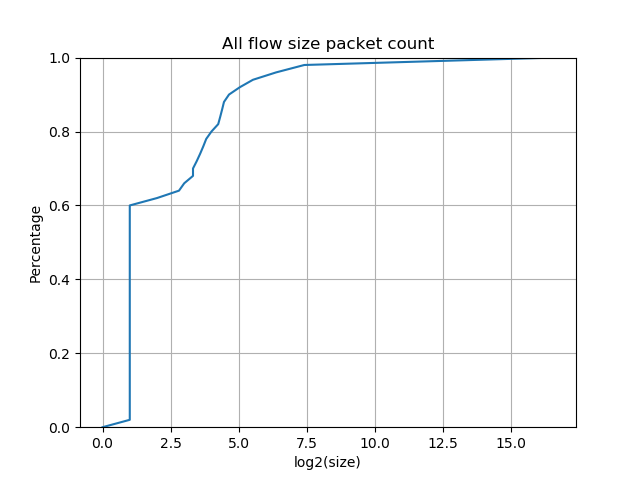
\includegraphics[width=0.9\linewidth]{graphs/All_flow_size_packet_count.png}
\end{subfigure}
\label{all_flow_size}
\end{figure*}
\begin{figure*}[ht]
\begin{subfigure}{.5\textwidth}
 \centering
  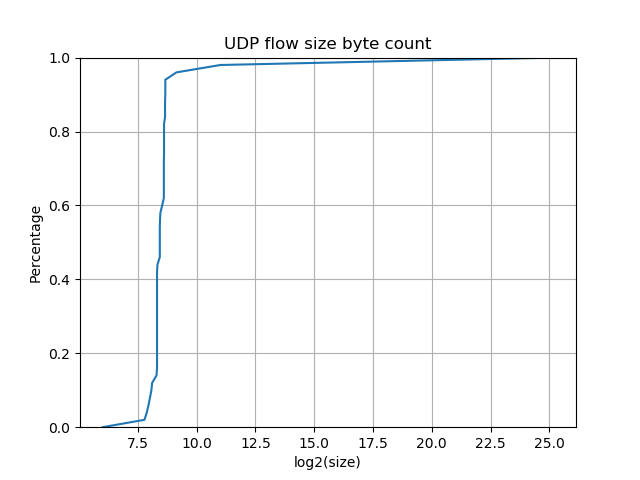
\includegraphics[width=0.9\linewidth]{graphs/UDP_flow_size_byte_count.png}
\end{subfigure}
\begin{subfigure}{.5\textwidth}
 \centering
  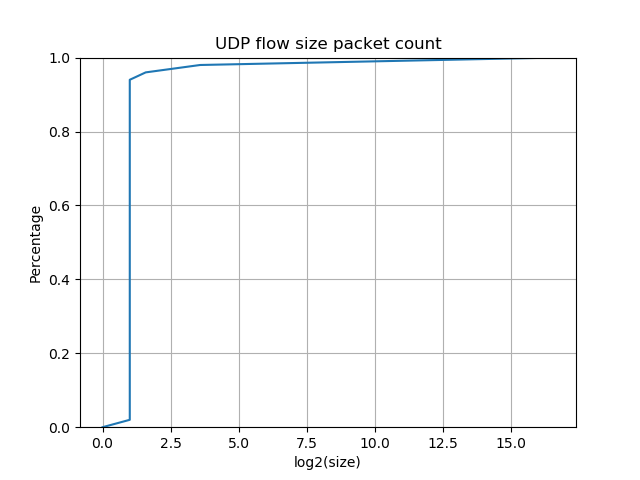
\includegraphics[width=0.9\linewidth]{graphs/UDP_flow_size_packet_count.png}
\end{subfigure}
\label{UDP_flow_size}
\end{figure*}
\begin{figure*}[ht]
\begin{subfigure}{.33\textwidth}
 \centering
  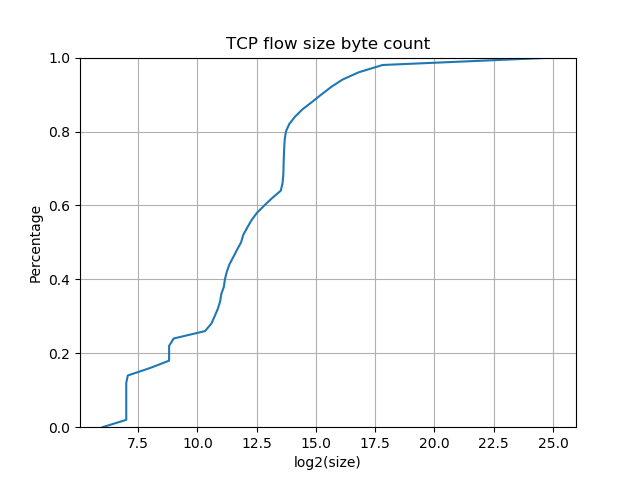
\includegraphics[width=1.1\linewidth]{graphs/TCP_flow_size_byte_count.png}
\end{subfigure}
\begin{subfigure}{.33\textwidth}
 \centering
  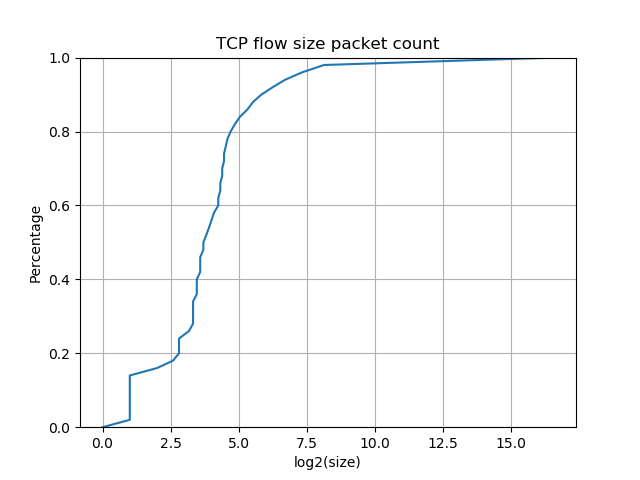
\includegraphics[width=1.1\linewidth]{graphs/TCP_flow_size_packet_count.png}
\end{subfigure}
\begin{subfigure}{.33\textwidth}
 \centering
  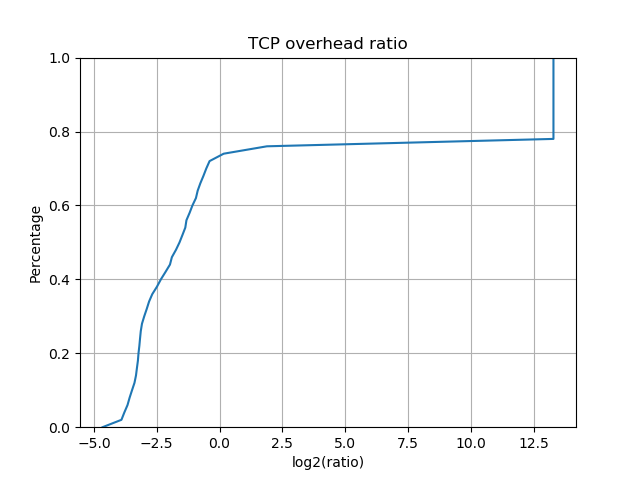
\includegraphics[width=1.1\linewidth]{graphs/TCP_overhead_ratio.png}
\end{subfigure}
\label{TCP_flow_size}
\end{figure*}

Inter-packet arrival time:\\
From the CDFs below, it is easily observable that most of the inter-arrival time a very close to 0. All three graphs demonstrate that only less than 5\% of the inter-arrival times are deviated from 0. And there are very long inter-arrival time for both TCP flows and UDP flows. There isn't much difference between TCP and UDP flows in terms of inter-arrival time. The only minor difference is that a little more UDP flows have longer inter-arrival time. Just as a notice, this inter-packet arrival time combined both direction.
\begin{figure*}[ht]
\begin{subfigure}{.33\textwidth}
 \centering
  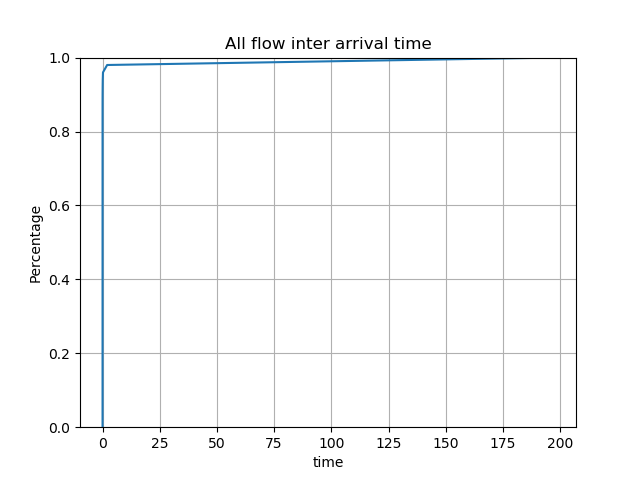
\includegraphics[width=1.1\linewidth]{graphs/All_flow_inter_arrival_time.png}
\end{subfigure}
\begin{subfigure}{.33\textwidth}
 \centering
  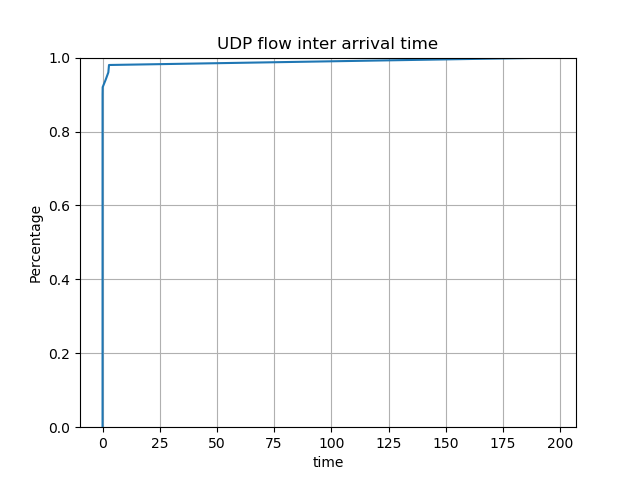
\includegraphics[width=1.1\linewidth]{graphs/UDP_flow_inter_arrival_time.png}
\end{subfigure}
\begin{subfigure}{.33\textwidth}
 \centering
  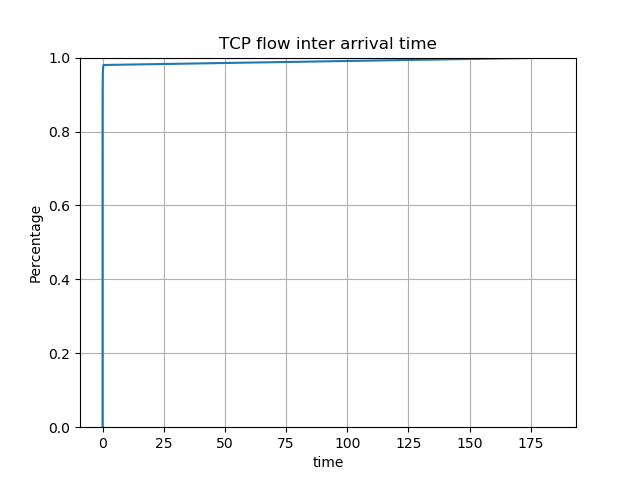
\includegraphics[width=1.1\linewidth]{graphs/TCP_flow_inter_arrival_time.png}
\end{subfigure}
\label{Inter-packet_arrival_time}
\end{figure*}

TCP State:\\
For some flows, both rst and fin are used to terminate the conversation. In those cases, I count them toward Finished if both side have send the fin and the fin is ACKed. If the process is not finished, I count them toward reset.
\begin{table}[h!]
\begin{tabular}{llllll}
                      & Request   & Reset  & Finished & Ongoing  & Failed \\
End State          & 144 	&3466   & 4938 & 925 & 0 \\
\end{tabular}
\end{table}

\end{homeworkProblem}
\clearpage
%----------------------------------------------------------------------------------------
%	PROBLEM 3
%----------------------------------------------------------------------------------------

\begin{homeworkProblem}
\noindent \textit{RTT Estimation}\\

Below are the graphes for the estimated RTT(SRTT) and sample RTT. The orange lines are estimated RTTs and the blue lines are the sample RTTs. When I calculate the RTT, I include the (FIN), (FIN,ACK) pair too. So my result is a little bit different from wiresharks. Notice that the 3 largest TCP flows in terms of packet number are also the 3 largest TCP flows in terms of total byte size.\\
In general, we can see that sample RTTs are really unstable, with large spikes and a lot of fluctuation. In contrast, the estimated RTTs are much more stable than the sample RTTs. They have smaller spikes and stays approximately at average of the sample RTTs. The reason is that we calculate the SRTTs are a weighted sum of SRTT and the sample RTT. A spike in RTT won't affect the SRTT in full scale.\\
There isn't a general patteren in how the RTTs changed. For example, for the flow with largest packet number and third largest total byte, the RTT was at first very unstable and larger in average and become smaller and more stable after 50s. This could the result of a better route being available after 50s, or it gets a priority because it is communicating more frequently, or the network is not as busy and have shorter queues. The flow with second largest packet number have an opposite behavior. This maybe a result of busier network and longer queues. For other flows, the SRTT and RTT's average remain similar throughout the life of the connection.\\
\begin{figure*}[ht]
\begin{subfigure}{.33\textwidth}
 \centering
  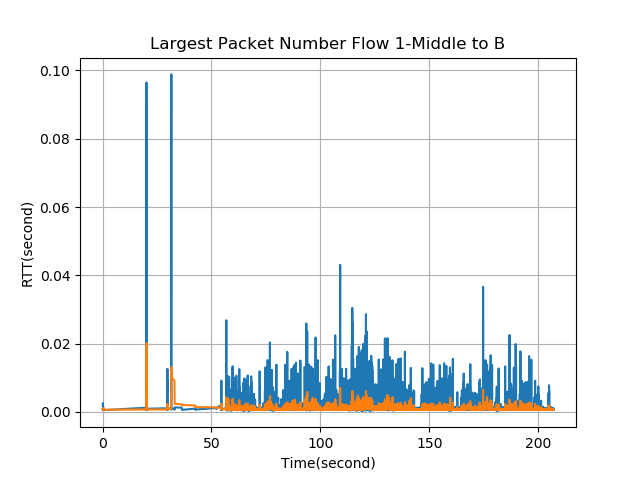
\includegraphics[width=1.1\linewidth]{graphs/Largest_Packet_Number_Flow_1-Middle_to_B.png}
\end{subfigure}
\begin{subfigure}{.33\textwidth}
 \centering
  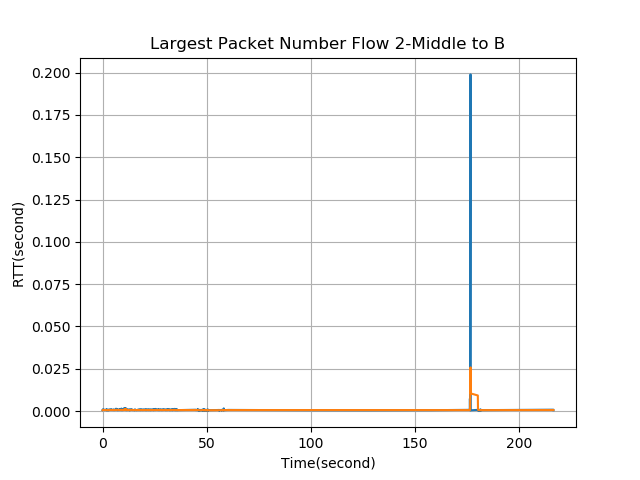
\includegraphics[width=1.1\linewidth]{graphs/Largest_Packet_Number_Flow_2-Middle_to_B.png}
\end{subfigure}
\begin{subfigure}{.33\textwidth}
 \centering
  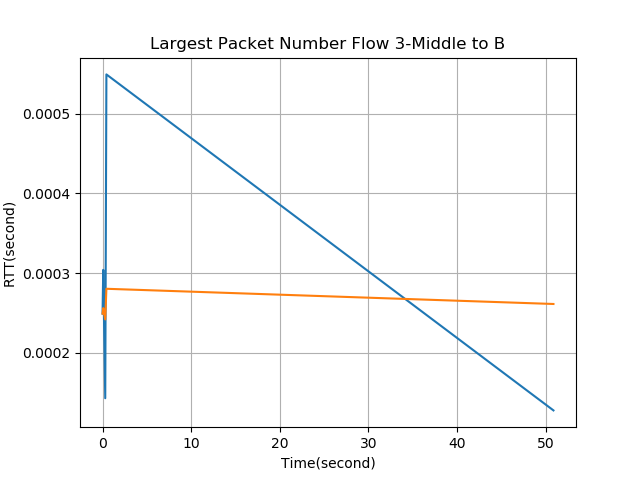
\includegraphics[width=1.1\linewidth]{graphs/Largest_Packet_Number_Flow_3-Middle_to_B.png}
\end{subfigure}
\begin{subfigure}{.33\textwidth}
 \centering
  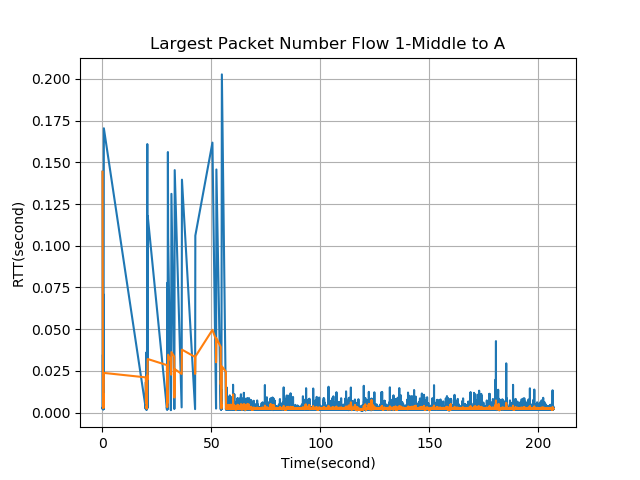
\includegraphics[width=1.1\linewidth]{graphs/Largest_Packet_Number_Flow_1-Middle_to_A.png}
\end{subfigure}
\begin{subfigure}{.33\textwidth}
 \centering
  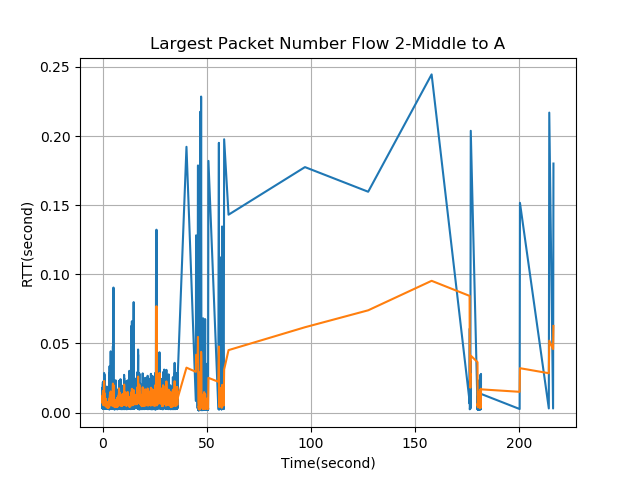
\includegraphics[width=1.1\linewidth]{graphs/Largest_Packet_Number_Flow_2-Middle_to_A.png}
\end{subfigure}
\begin{subfigure}{.33\textwidth}
 \centering
  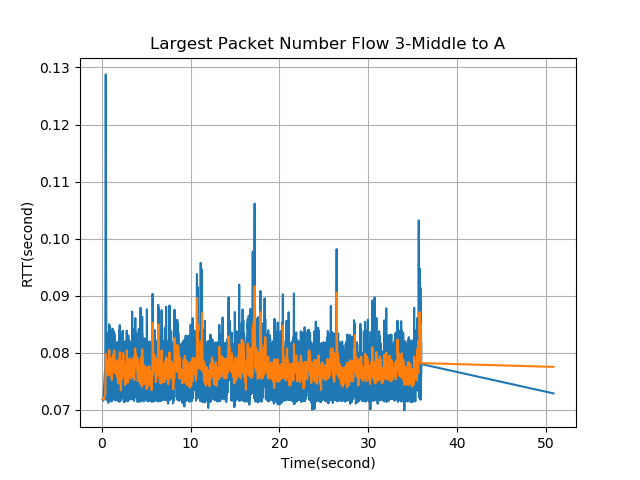
\includegraphics[width=1.1\linewidth]{graphs/Largest_Packet_Number_Flow_3-Middle_to_A.png}
\end{subfigure}
\end{figure*}

\begin{figure*}[ht]
\begin{subfigure}{.33\textwidth}
 \centering
  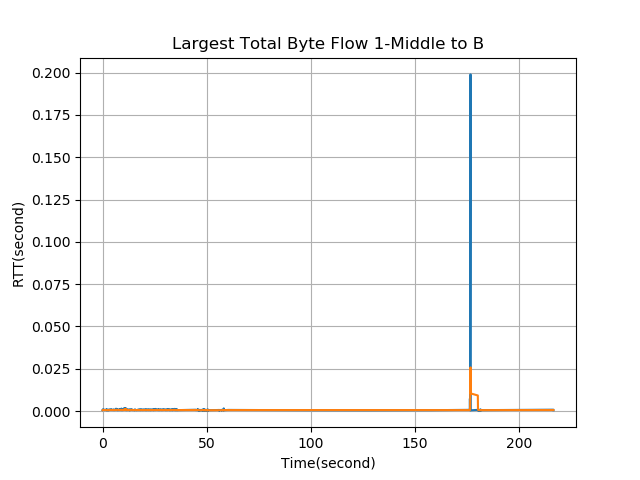
\includegraphics[width=1.1\linewidth]{graphs/Largest_Total_Byte_Flow_1-Middle_to_B.png}
\end{subfigure}
\begin{subfigure}{.33\textwidth}
 \centering
  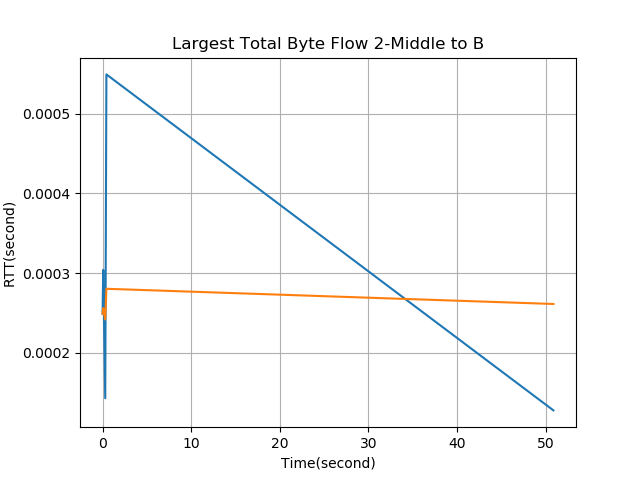
\includegraphics[width=1.1\linewidth]{graphs/Largest_Total_Byte_Flow_2-Middle_to_B.png}
\end{subfigure}
\begin{subfigure}{.33\textwidth}
 \centering
  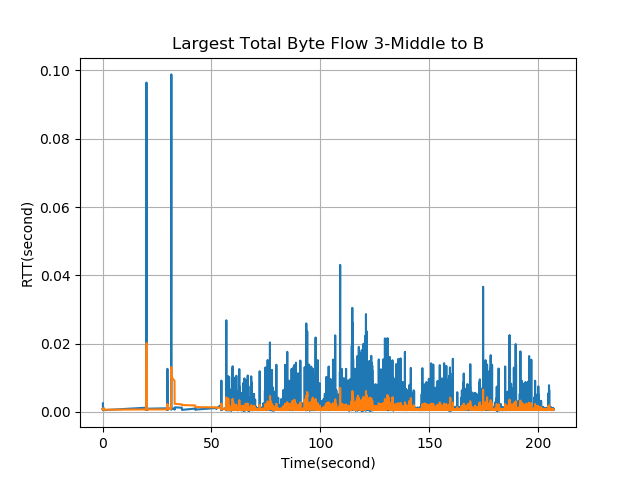
\includegraphics[width=1.1\linewidth]{graphs/Largest_Total_Byte_Flow_3-Middle_to_B.png}
\end{subfigure}
\begin{subfigure}{.33\textwidth}
 \centering
  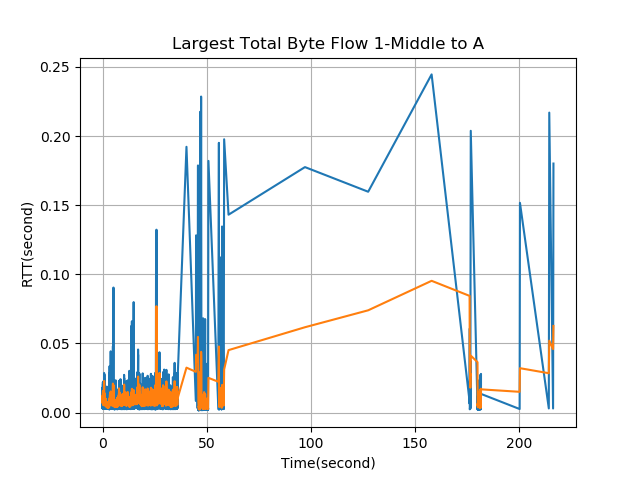
\includegraphics[width=1.1\linewidth]{graphs/Largest_Total_Byte_Flow_1-Middle_to_A.png}
\end{subfigure}
\begin{subfigure}{.33\textwidth}
 \centering
  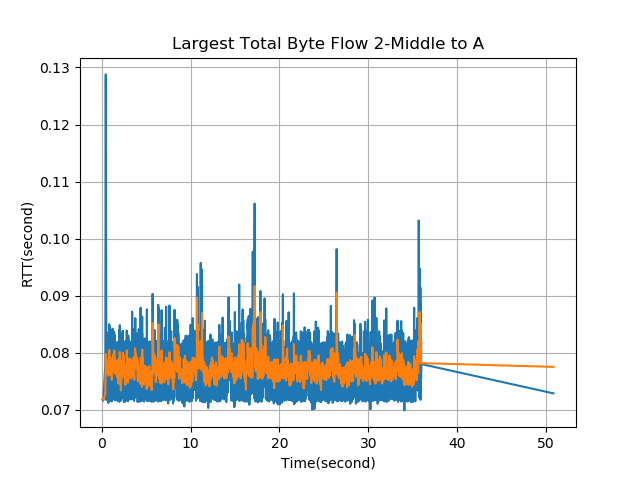
\includegraphics[width=1.1\linewidth]{graphs/Largest_Total_Byte_Flow_2-Middle_to_A.png}
\end{subfigure}
\begin{subfigure}{.33\textwidth}
 \centering
  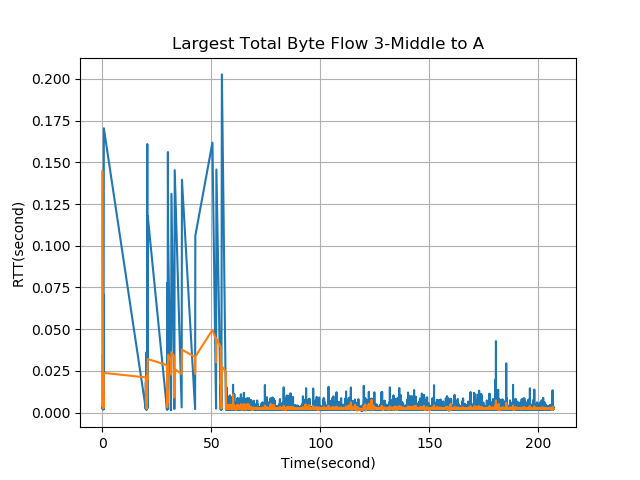
\includegraphics[width=1.1\linewidth]{graphs/Largest_Total_Byte_Flow_3-Middle_to_A.png}
\end{subfigure}
\begin{subfigure}{.33\textwidth}
 \centering
  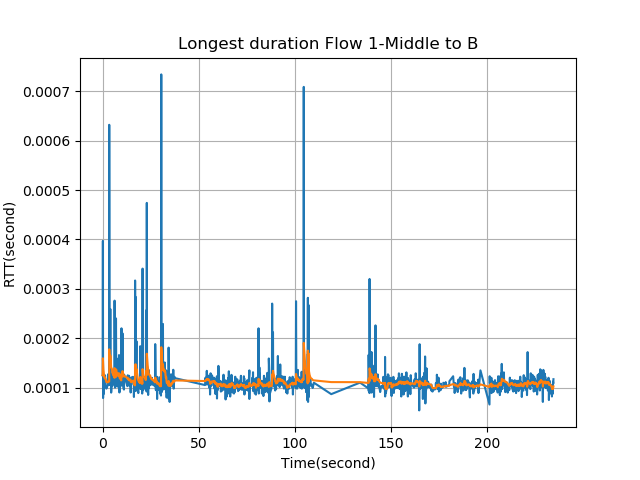
\includegraphics[width=1.1\linewidth]{graphs/Longest_duration_Flow_1-Middle_to_B.png}
\end{subfigure}
\begin{subfigure}{.33\textwidth}
 \centering
  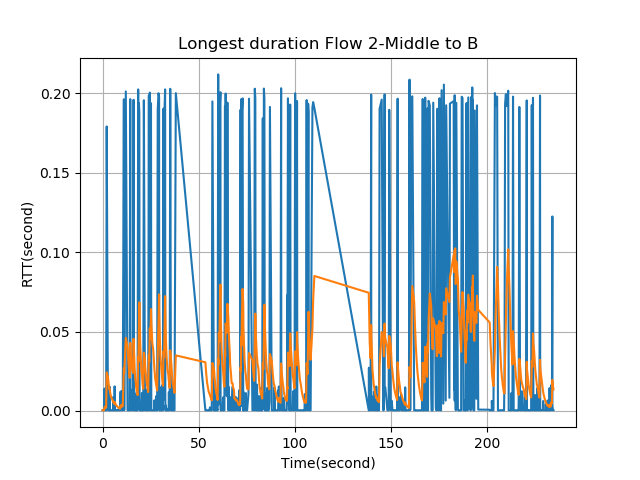
\includegraphics[width=1.1\linewidth]{graphs/Longest_duration_Flow_2-Middle_to_B.png}
\end{subfigure}
\begin{subfigure}{.33\textwidth}
 \centering
  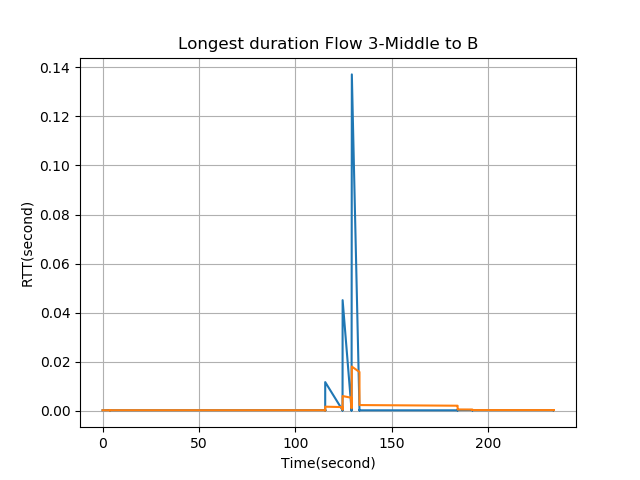
\includegraphics[width=1.1\linewidth]{graphs/Longest_duration_Flow_3-Middle_to_B.png}
\end{subfigure}
\begin{subfigure}{.33\textwidth}
 \centering
  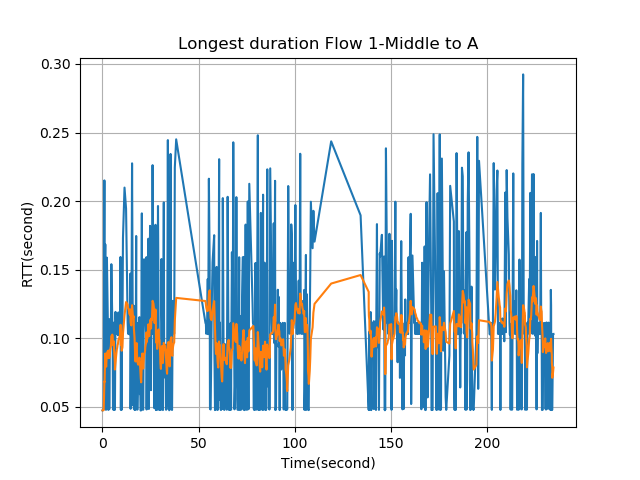
\includegraphics[width=1.1\linewidth]{graphs/Longest_duration_Flow_1-Middle_to_A.png}
\end{subfigure}
\begin{subfigure}{.33\textwidth}
 \centering
  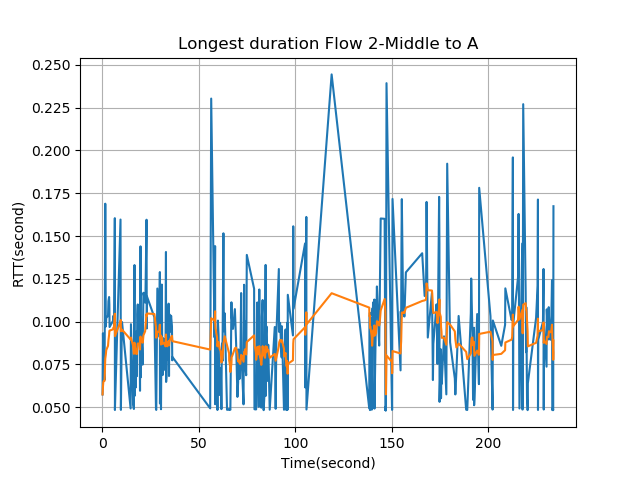
\includegraphics[width=1.1\linewidth]{graphs/Longest_duration_Flow_2-Middle_to_A.png}
\end{subfigure}
\begin{subfigure}{.33\textwidth}
 \centering
  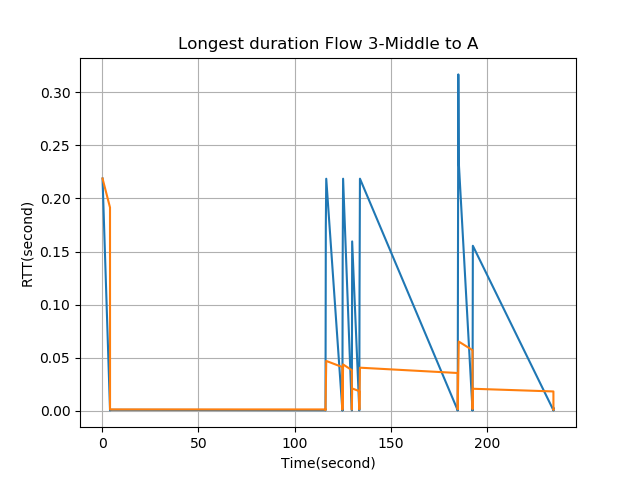
\includegraphics[width=1.1\linewidth]{graphs/Longest_duration_Flow_3-Middle_to_A.png}
\end{subfigure}
\label{Longest_duration_flow}
\label{Longest_duration_flow}
\end{figure*}

\end{homeworkProblem}
\clearpage
%----------------------------------------------------------------------------------------
%	PROBLEM 4
%----------------------------------------------------------------------------------------

\begin{homeworkProblem}
\noindent \textit{RTT Estimation change from time to time}\\
\\

The three pair of hosts are (244.3.160.204, 244.3.160.254),  (244.3.160.204, 244.3.160.89), (244.3.160.204, 244.3.160.239). Notice that all three pairs of hosts have 244.3.160.204 and their connections all span the whole 240 second of the pcap file.\\
(244.3.160.204, 244.3.160.254): There isn't a pattern for RTTs between middle and 244.3.160.254. The representative RTTs fluctuates in a small range, with some large spikes. For RTTs between middle and 244.3.160.204, we can observe that between 100s and 200s, the RTTs are shorter in average, and then return to previous level after 200s. This reason could be the route between middle and 244.3.160.204 is less congested, with less queueing time, or a better route is available only during that period\\
(244.3.160.204, 244.3.160.89): For RTTs between middle and 244.3.160.89, again it is only some random minor changes with large spikes. And the conclusion of the RTTs between middle and 244.3.160.204 is similar to previous pair.\\
(244.3.160.204, 244.3.160.239): For RTTs between middle and 244.3.160.239, it is still some random minor changes with large spikes. And the conclusion of the RTTs between middle and 244.3.160.204 is similar to previous pair.\\
All 3 together: Lets say 244.3.160.204 is A and the other ones are B1, B2, B3. The RTTs between middle and B1, B2, B3 are different. They have spikes at different time. This is happening because it takes different route from collection point to B1, B2, B3. So the spike may happen on a router that is not shared by the three routes. As a contrast the three graphs of RTTs between middle and A is almost identical. This is because the route used between middle and A is probably the same. And thus when there is a spike, it will appears in all three graphs.
\begin{figure*}[ht]
\begin{subfigure}{.33\textwidth}
 \centering
  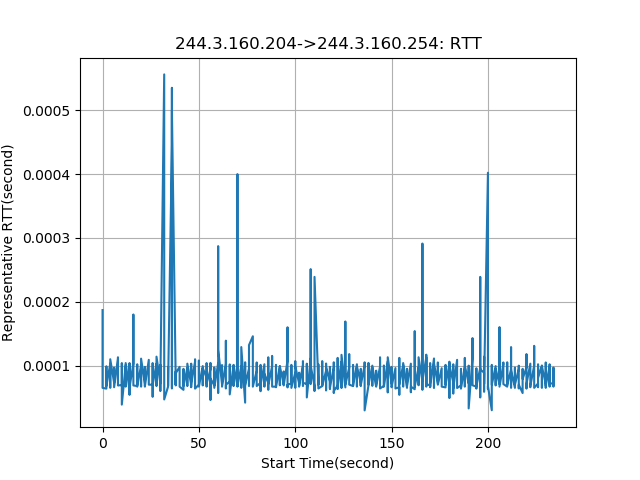
\includegraphics[width=1.1\linewidth]{graphs/Top_3_Pair_of_Hosts_1-a2b.png}
\end{subfigure}
\begin{subfigure}{.33\textwidth}
 \centering
  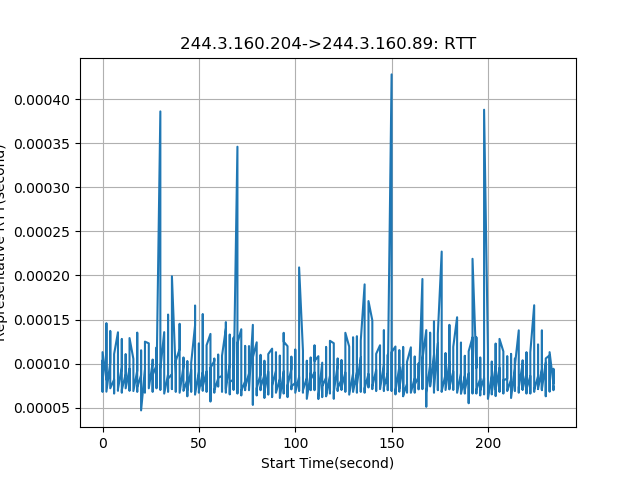
\includegraphics[width=1.1\linewidth]{graphs/Top_3_Pair_of_Hosts_2-a2b.png}
\end{subfigure}
\begin{subfigure}{.33\textwidth}
 \centering
  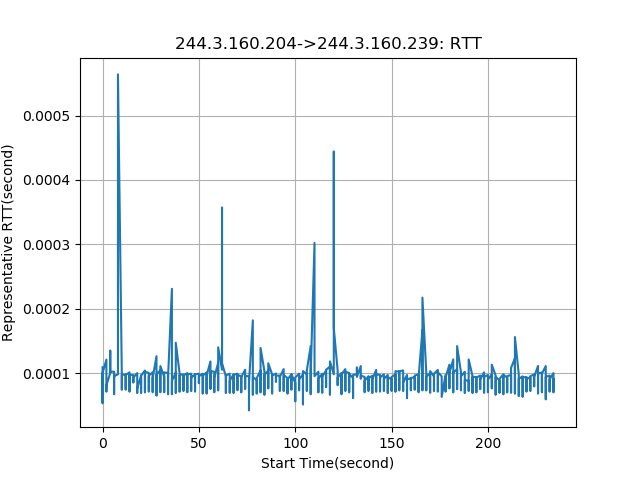
\includegraphics[width=1.1\linewidth]{graphs/Top_3_Pair_of_Hosts_3-a2b.png}
\end{subfigure}
\begin{subfigure}{.33\textwidth}
 \centering
  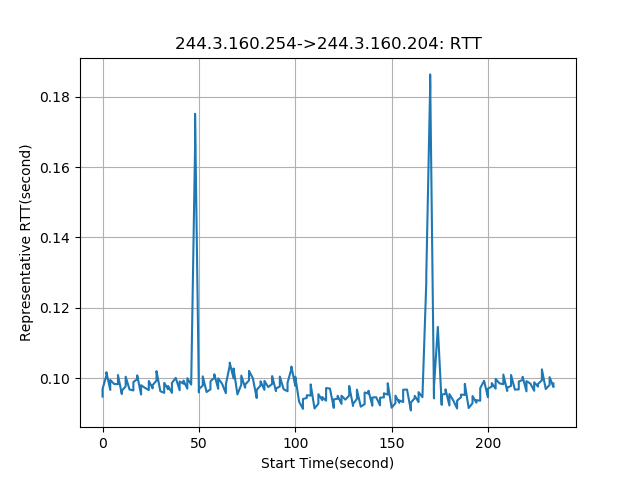
\includegraphics[width=1.1\linewidth]{graphs/Top_3_Pair_of_Hosts_1-b2a.png}
\end{subfigure}
\begin{subfigure}{.33\textwidth}
 \centering
  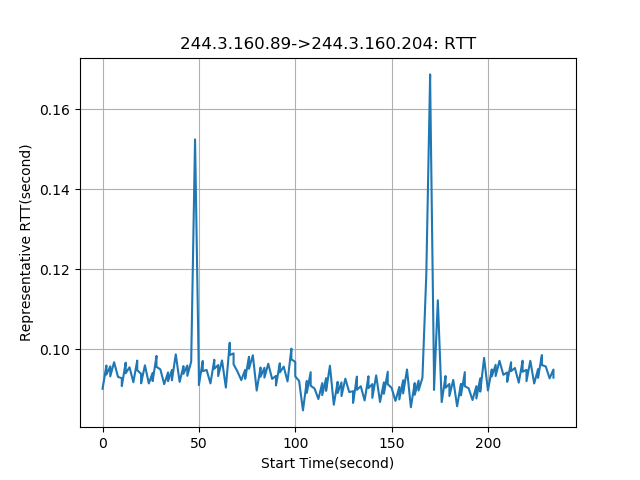
\includegraphics[width=1.1\linewidth]{graphs/Top_3_Pair_of_Hosts_2-b2a.png}
\end{subfigure}
\begin{subfigure}{.33\textwidth}
 \centering
  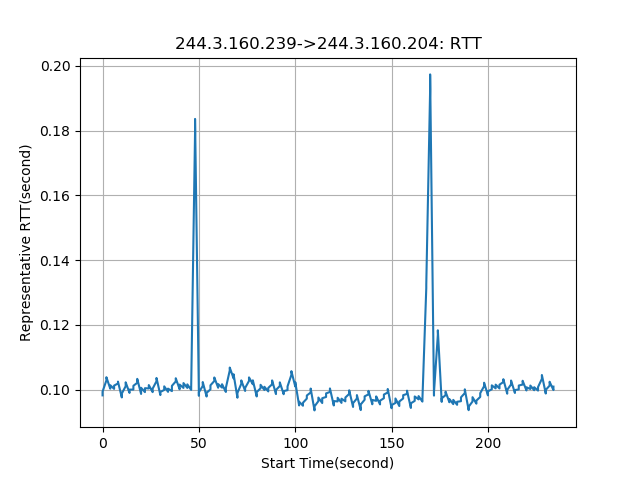
\includegraphics[width=1.1\linewidth]{graphs/Top_3_Pair_of_Hosts_3-b2a.png}
\end{subfigure}
\label{Inter-packet_arrival_time}
\end{figure*}

\end{homeworkProblem}
%----------------------------------------------------------------------------------------

\end{document}
